% !TeX root = 11Javier_TARAZONA_CV_Safran_IACloud.tex
% !TeX program = pdflatex
%-------------------------
% Resume in Latex
% Author : Javier Tarazona
%------------------------

\documentclass[letterpaper,10pt]{article}
\DeclareUnicodeCharacter{00A0}{~}
\DeclareUnicodeCharacter{2013}{\textendash}
\DeclareUnicodeCharacter{2014}{\textemdash}
\DeclareUnicodeCharacter{201C}{``}
\DeclareUnicodeCharacter{201D}{''}
\DeclareUnicodeCharacter{2022}{\textbullet}
\DeclareUnicodeCharacter{25E6}{\textopenbullet}
% \setlist[itemize]{label=\textbullet, labelsep=0.5em, leftmargin=*} % Moved after \begin{document}
\usepackage[T1]{fontenc}      % Codificación de salida (acentos y símbolos)
\usepackage[empty]{fullpage}
\usepackage[export]{adjustbox}
\usepackage[pdftex]{hyperref}
\usepackage[usenames,dvipsnames]{color}
\usepackage[utf8]{inputenc}   % Lee texto en UTF-8
\usepackage{array}
\usepackage{comment}
\usepackage{enumitem}
\usepackage{enumitem}         % Control de listas (si no lo tienes ya)
\usepackage{fancyhdr}
\usepackage{graphicx}
\usepackage{latexsym}
\usepackage{lmodern}
\usepackage{marvosym}
\usepackage{tabularx}
\usepackage{titlesec}
\usepackage{verbatim}
\usepackage{xcolor}


\usepackage{latexsym}
\usepackage[empty]{fullpage}
\usepackage{titlesec}
\usepackage{marvosym}
\usepackage[usenames,dvipsnames]{color}
\usepackage{verbatim}
\usepackage{enumitem}
\usepackage[pdftex]{hyperref}
\usepackage{fancyhdr}
\usepackage{tabularx}
\usepackage{graphicx}
\usepackage{array}
\usepackage[export]{adjustbox}
\usepackage{xcolor}
\usepackage{comment}

\begin{comment}
\end{comment}
% --- Codificación y fuentes seguras ---
\usepackage[utf8]{inputenc}   % Lee texto en UTF-8
\usepackage[T1]{fontenc}      % Codificación de salida (acentos y símbolos)
\usepackage{enumitem}         % Control de listas (si no lo tienes ya)

% --- Viñetas limpias y seguras ---
\setlist[itemize]{label=\textbullet, labelsep=0.5em, leftmargin=*}
%\end{comment}

\pagestyle{empty}

% Adjust margins
\addtolength{\oddsidemargin}{-0.45in}
\addtolength{\evensidemargin}{-0.45in}
\addtolength{\textwidth}{1.15in}
\addtolength{\topmargin}{-.62in}
\addtolength{\textheight}{1.20in}

\urlstyle{same}

\raggedbottom
\raggedright
\setlength{\tabcolsep}{0in}
\renewcommand{\arraystretch}{0.98}

%\definecolor{mydarkgreen}{RGB}{0, 140, 123}
\definecolor{mydarkgreen}{RGB}{0, 0, 0}

% Sections formatting
\titleformat{\section}{
  \vspace{-3pt}\scshape\raggedright\large
}{}{0em}{}[\color{mydarkgreen}\titlerule \vspace{-5pt}]

%-------------------------
% Custom commands
\newcommand{\resumeItemCompact}[2]{\item\small{\textbf{#1}: #2}\vspace{-2pt}}
\newcommand{\resumeItemListStartCompact}{\begin{itemize}[leftmargin=*,itemsep=0pt,parsep=0pt,topsep=0pt,partopsep=0pt,nolistsep]}
\newcommand{\resumeItemListEndCompact}{\end{itemize}\vspace{-4pt}}

\newcommand{\resumeItem}[2]{
  \item\small{
    \textbf{#1}{: #2 \vspace{-2pt}}
  }
}

\newcommand{\resumeSubheading}[4]{
  \vspace{-1pt}\item
    \begin{tabular*}{0.97\textwidth}{l@{\extracolsep{\fill}}r}
      	\textbf{#1} & \textbf{\textcolor{mydarkgreen}{#2}} \\
      	\textit{\footnotesize#3} & \textit{\footnotesize \textcolor{mydarkgreen}{#4}} \\
    \end{tabular*}\vspace{-4pt}
}

\newcommand{\resumeSubItem}[2]{\resumeItem{#1}{#2}\vspace{-4pt}}

\renewcommand{\labelitemii}{$\circ$}

\newcommand{\resumeSubHeadingListStart}{\begin{itemize}[leftmargin=*]}
\newcommand{\resumeSubHeadingListEnd}{\end{itemize}}
\newcommand{\resumeItemListStart}{\begin{itemize}[itemsep=0pt,parsep=0pt,topsep=0pt,partopsep=0pt]}
\newcommand{\resumeItemListEnd}{\end{itemize}\vspace{-5pt}}

% Indented paragraph helper: \indentbox[ancho]{contenido}
% Uso: \indentbox{Texto...}  o  \indentbox[1.5em]{Texto...}
\newcommand{\indentbox}[2][1em]{\hspace*{#1}\parbox{\dimexpr\linewidth-#1\relax}{#2}}

\newlength{\headerPhotoSpace}
\setlength{\headerPhotoSpace}{0pt}
\newcommand{\showHeaderPhoto}{%
  \setlength{\headerPhotoSpace}{0.13\textwidth}%
  \makebox[0pt][l]{\adjustbox{valign=c}{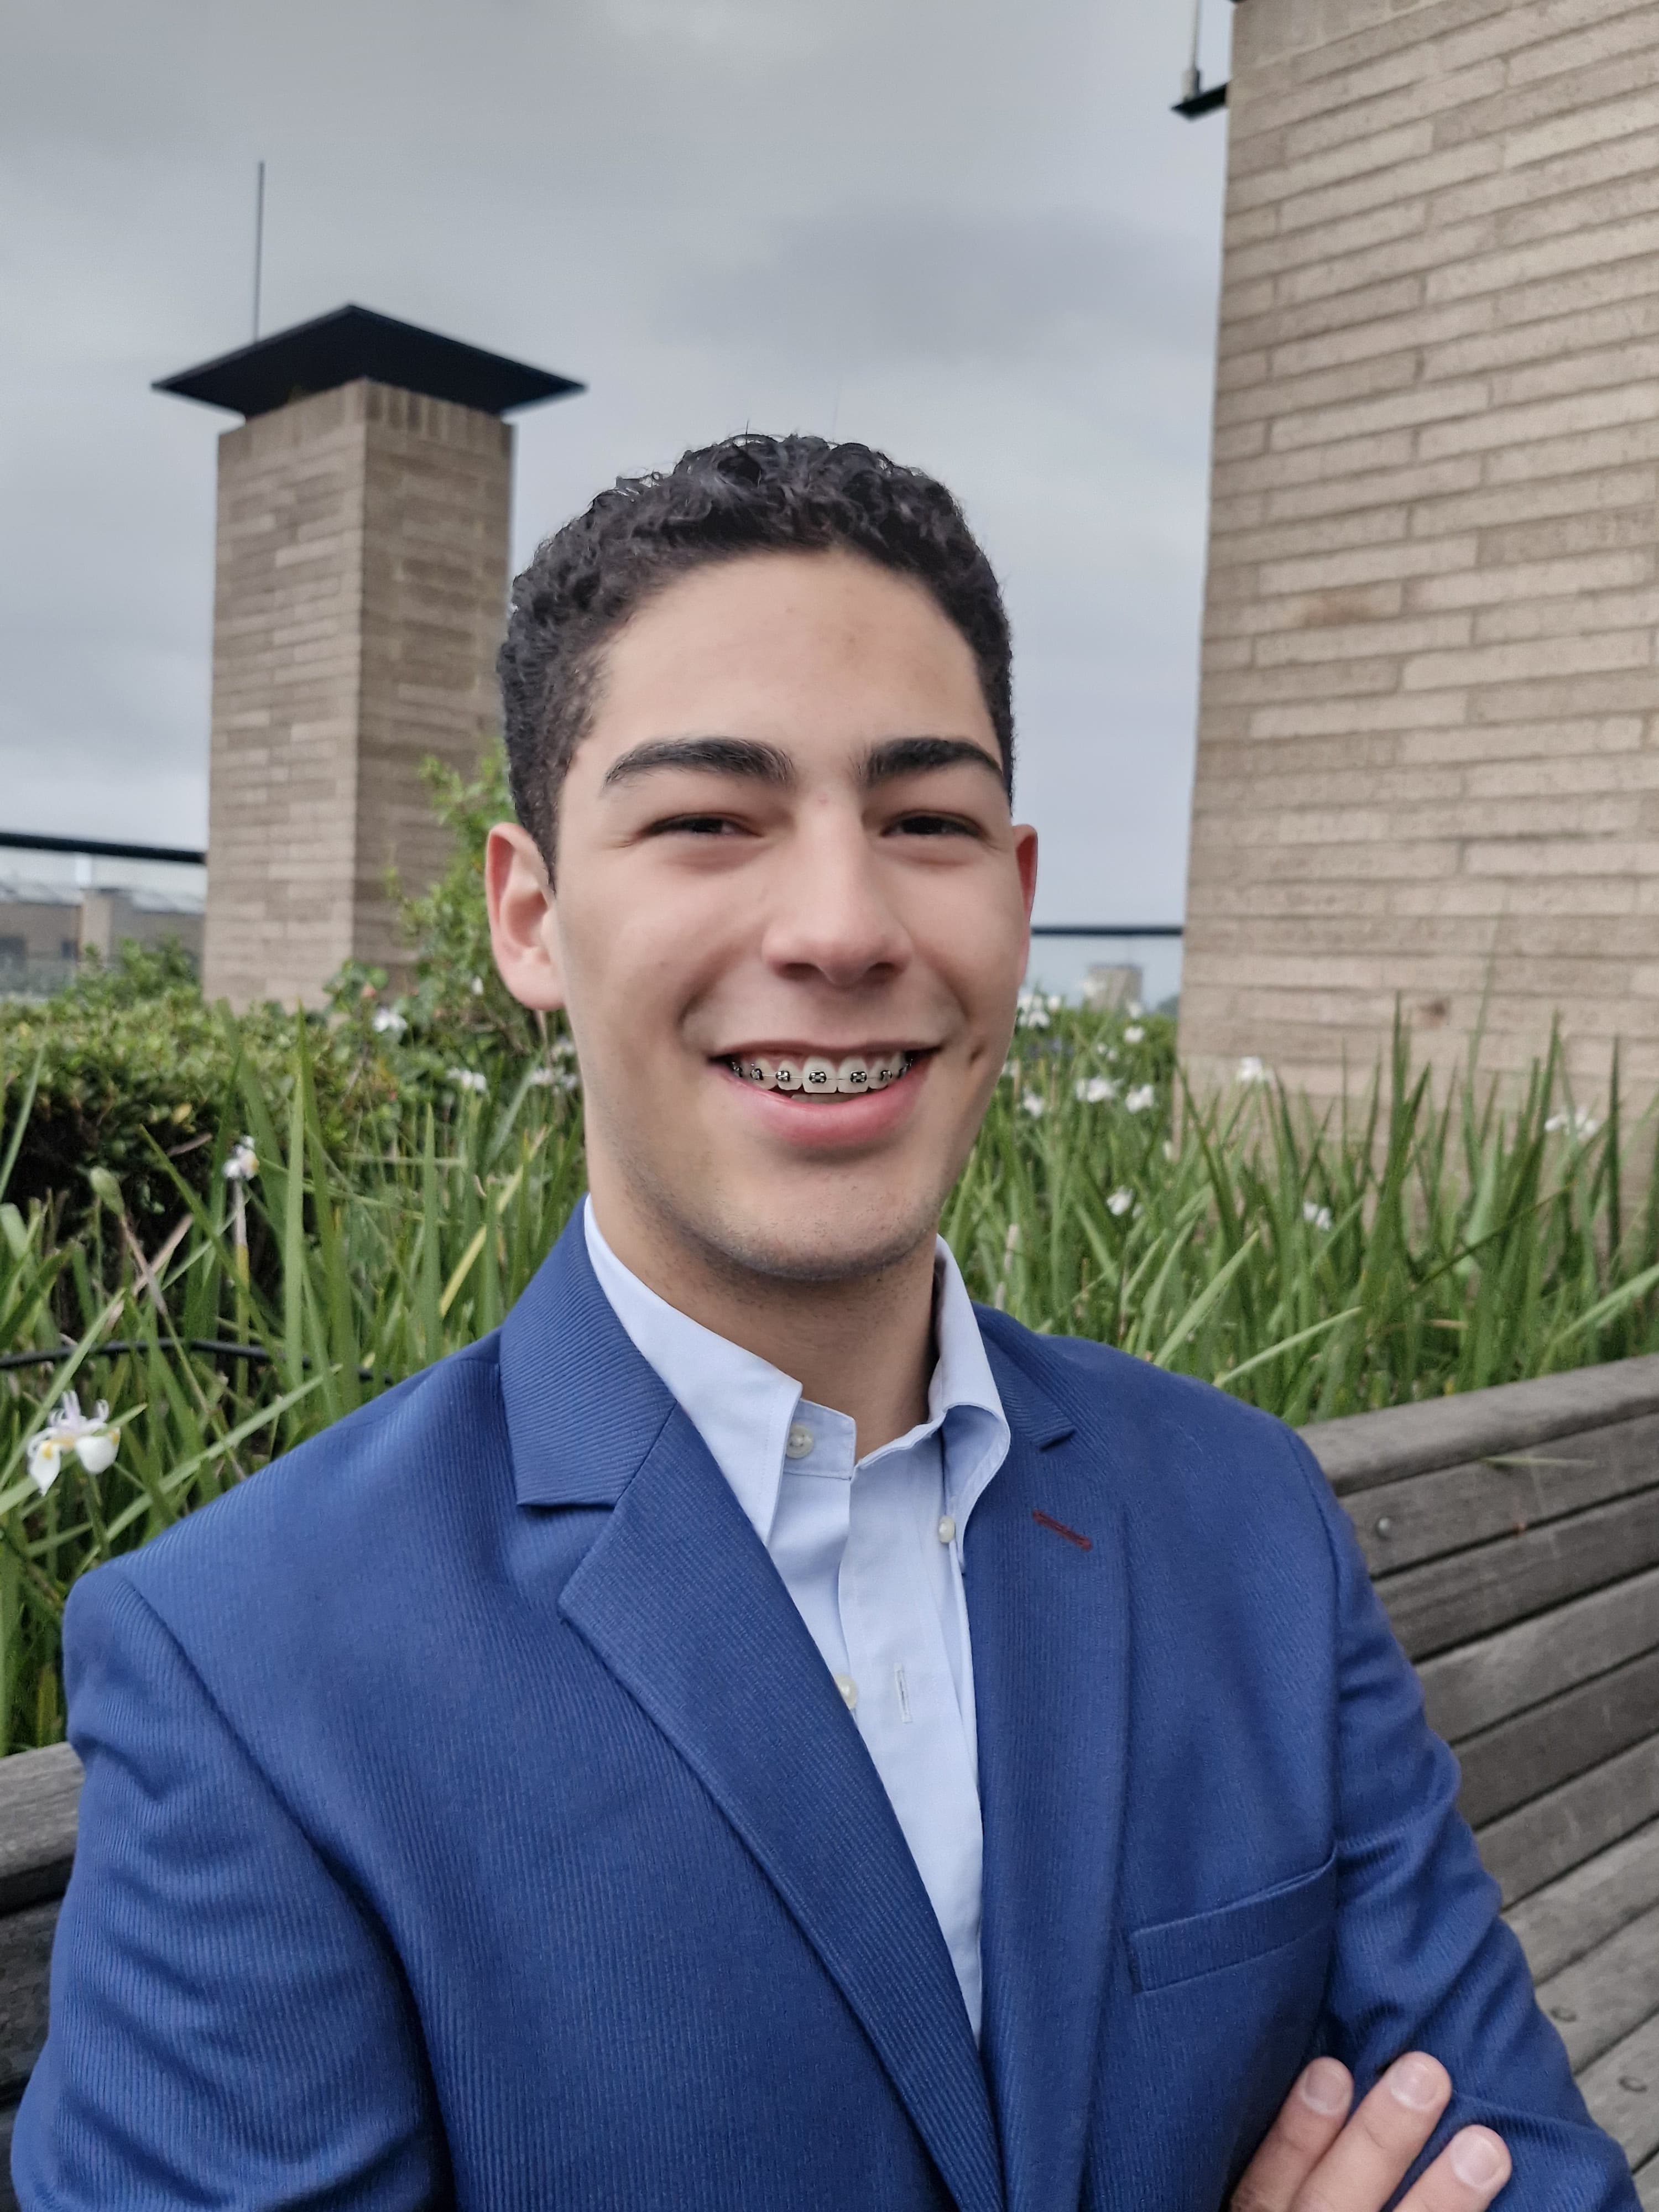
\includegraphics[scale=0.015]{Digital_photo.jpg}}}%
}


%-------------------------------------------
%%%%%%  CV STARTS HERE  %%%%%%%%%%%%%%%%%%%%%%%%%%%%


\begin{document}

\begin{comment}
\AddToHookNext{shipout/foreground}{%
  \put(\dimexpr\paperwidth-0.35cm\relax,-\dimexpr\paperheight-0.35cm\relax){%
    \makebox(0,0)[rb]{%
      \begin{minipage}{2.15cm}
        \centering
        {\setlength{\fboxsep}{1pt}\colorbox{white}{%
          \parbox{1.9cm}{\centering\scriptsize\bfseries Scannez le QR \\[-1pt]pour la version numérique}}}\\[1pt]
        
\includegraphics[width=1.6cm]{qr_CV.png}%
      \end{minipage}%
    }%
  }%
}
\end{comment}

% --- Viñetas limpias y seguras ---
\setlist[itemize]{label=\textbullet, labelsep=0.5em, leftmargin=*}

%----------HEADING-----------------

\noindent
%\showHeaderPhoto% Commenter cette ligne pour retirer la photo et élargir l'en-tête.
\hspace*{\headerPhotoSpace}%
\begin{minipage}[c]{\dimexpr\textwidth-\headerPhotoSpace\relax}
  \begin{tabular*}{\linewidth}{@{}l@{\extracolsep{\fill}}r@{}}

            \textbf{\Large \textcolor{mydarkgreen}{Javier Andres TARAZONA JIMENEZ}} & \textbf{\textcolor{mydarkgreen}{Email:}} \href{mailto:javitar06@gmail.com}{javitar06@gmail.com}\\

            \footnotesize \'Etudiant Ing\'enieur Bac+5 \textendash{} Double Dipl\^ome ENSTA Paris / UNAL & \href{mailto:javier-andres.tarazona@ensta-paris.fr}{javier-andres.tarazona@ensta-paris.fr}\\
            \footnotesize Data Engineering, IA g\'en\'erative, NLP/LLMs, API, Pipelines, Cloud & \textbf{\textcolor{mydarkgreen}{Mobile:}} +33 07 46 36 97 75 \\

            \href{https://www.linkedin.com/in/javier-andres-tarazona-jimenez-84b489222/}{\textcolor{blue}{\underline{LinkedIn}}} & Massy, \^Ile de France, France (91300)\\

            \href{https://github.com/JavierTarazona06}{\textcolor{blue}{\underline{GitHub}}} & \\
        \end{tabular*}
\end{minipage}

\vspace{0.15cm}

\textbf{Recherche une alternance de derni\`ere ann\'ee \textendash{} Data Engineering \& IA Cloud (AWS), \`a partir de septembre 2026}


\vspace{0.02cm}

%-----------FORMATION-----------------
\section{\textcolor{mydarkgreen}{\textbf{FORMATION}}}

\begin{tabularx}{\textwidth}{>{\raggedright\arraybackslash}X >{\raggedleft\arraybackslash}p{0.24\textwidth}}
  \begin{minipage}[t]{\linewidth}\raggedright
  \textbullet\ \textbf{Institut Polytechnique de Paris (IPP) - ENSTA}\\
  \textit{\footnotesize Dipl\^ome d'Ing\'enieur - Master of Science in Engineering - Ax\'e sur IA}\\
  \textit{\footnotesize Cours Pertinents : Machine Learning, Bases de Donn\'ees, G\'enie Logiciel, R\'eseaux, Syst\`emes Distribu\'es}
  \end{minipage}
  &
  \begin{minipage}[t]{\linewidth}\raggedleft
  \textbf{Paris, France}\\
  {\footnotesize\textit{Septembre 2025 -- Pr\'esent}}
  \end{minipage}
  \\
  \begin{minipage}[t]{\linewidth}
  \textbullet\ \textbf{Universidad Nacional de Colombia (UNAL)}\\
  \textit{\footnotesize Ing\'enierie des Syst\`emes et Informatique}\\
  \textit{\footnotesize Cours Pertinents : G\'enie Logiciel I/II, Bases de Donn\'ees, Syst\`emes d'Information, R\'eseaux, Structures de Donn\'ees}
  \end{minipage}
  &
  \begin{minipage}[t]{\linewidth}\raggedleft
  \textbf{Bogot\'a, Colombie}\\
  {\footnotesize\textit{Janvier 2021 -- Juillet 2025}}
  \end{minipage}
  \\
  \begin{minipage}[t]{\linewidth}
  \textbullet\ \textbf{University of Saskatchewan}\\
  \textit{\footnotesize \'Echange acad\'emique.}\\
  \textit{\footnotesize Cours : Ing\'enierie logicielle, Algorithmes, Syst\`emes d'exploitation et Fran\c{c}ais des Affaires}
  \end{minipage}
  &
  \begin{minipage}[t]{\linewidth}\raggedleft
  \textbf{Saskatoon, Canada}\\
  {\footnotesize\textit{Septembre 2024 -- D\'ecembre 2024}}
  \end{minipage}
\end{tabularx}

\vspace{0.14cm}
%--------DISTINCTIONS------------
\section{\textcolor{mydarkgreen}{\textbf{DISTINCTIONS}}}

\begin{tabularx}{\textwidth}{
  % Suma de anchos: 0.75 + 1.45 + 0.80 = 3.00
  >{\hsize=0.77\hsize\linewidth=\hsize\raggedright\arraybackslash}X
  >{\hsize=1.33\hsize\linewidth=\hsize\raggedright\arraybackslash}X
  >{\hsize=0.90\hsize\linewidth=\hsize\raggedright\arraybackslash}X}
    \begin{minipage}[t]{\linewidth}\raggedright
      \textbullet\ \textbf{\textbf{Bourse Eiffel Excellence}}\\
      \textit{\footnotesize ENSTA - Master 2025\textendash{}2027}\\
    \end{minipage}
    &
    \begin{minipage}[t]{\linewidth}\raggedright
      \textbullet\ \textbf{Mention d'Honneur \textendash{} ICPC Colombie 2023}\\
      {\footnotesize\textit{XXXVII Marathon National de Programmation ACIS REDIS}}
    \end{minipage}
    &
    \begin{minipage}[t]{\linewidth}\raggedright
      \textbullet\ \textbf{Excellence acad\'emique}\\
      {\footnotesize\textit{UNAL - Exon\'eration des frais de scolarit\'e}}
    \end{minipage}\\
\end{tabularx}


\vspace{0.14cm}
%-----------EXPERIENCE-----------------
\section{\textcolor{mydarkgreen}{\textbf{EXP\'ERIENCE PROFESSIONNELLE}}}
  \begin{tabularx}{\textwidth}{>{\raggedright\arraybackslash}X >{\raggedleft\arraybackslash}p{0.4\textwidth}}

    \begin{minipage}[t]{\linewidth}\raggedright
      \textbullet\ \textbf{ENSTA Paris -- U2IS}\\
      \textit{\footnotesize Stagiaire de recherche en Intelligence Artificielle et Vision 3D}\\
    \end{minipage}
    &
    \begin{minipage}[t]{\linewidth}\raggedleft
      \textbf{Palaiseau, France}\\
      {\footnotesize\textit{Mai 2026 -- Pr\'esent}}
    \end{minipage}\\

    \multicolumn{2}{l}{
      \begin{minipage}[t]{\linewidth}\raggedright
        \indentbox{\footnotesize \textbf{- Pipeline de donn\'ees synth\'etiques :} G\'en\'eration automatis\'ee d'un dataset 3D (\textbf{Python/Blender}) : rendu multi-vues, cam\'eras, m\'etadonn\'ees ; structuration des donn\'ees pour l'entra\^inement IA (\textbf{curriculum learning}).}
      \end{minipage}
    }\\

    \multicolumn{2}{l}{
      \begin{minipage}[t]{\linewidth}\raggedright
        \indentbox{\footnotesize \textbf{- Entra\^inement deep learning :} Pr\'e-entra\^inement auto-supervis\'e (\textbf{PyTorch, Vision Transformers}) sur donn\'ees synth\'etiques pour apprendre la structure 3D.}
      \end{minipage}
    }\\

    %------------------------------------

    \begin{minipage}[t]{\linewidth}\raggedright
      \textbullet\ \textbf{APEDYS91}\\
      \textit{\footnotesize Machine Learning / NLP Engineer}\\
    \end{minipage}
    &
    \begin{minipage}[t]{\linewidth}\raggedleft
      \textbf{Paris, France}\\
      {\footnotesize\textit{Octobre 2025 - F\'evrier 2026}}
    \end{minipage}\\

    \multicolumn{2}{l}{
    \begin{minipage}[t]{\linewidth}\raggedright
        \indentbox{\footnotesize \textbf{- NLP \& LLMs locaux :} Pipeline de correction de texte fran\c{c}ais (\textbf{spaCy, LanguageTool, LLMs locaux}) avec guardrails NER, contr\^oles entit\'es/nombres et s\'election dynamique selon ressources mat\'erielles.}
    \end{minipage}
    }\\

    %------------------------------------

    \begin{minipage}[t]{\linewidth}\raggedright
      \textbullet\ \textbf{Engin A.I}\\
      \textit{\footnotesize Ing\'enieur Logiciel et Vision par Ordinateur}\\
    \end{minipage}
    &
    \begin{minipage}[t]{\linewidth}\raggedleft
      \textbf{Colombie - \'Etats-Unis}\\
      {\footnotesize\textit{12 mois : Jan. - Juil. 2024 et F\'ev. - Juin 2025}}
    \end{minipage}\\

    \multicolumn{2}{l}{
      \begin{minipage}[t]{\linewidth}\raggedright
        \indentbox{\footnotesize \textbf{- Architecture logicielle \& pipelines de donn\'ees :} Refactorisation en architecture modulaire/objet (\textbf{+70\,\% maintenabilit\'e}) ; optimisation de pipelines de traitement d'images (\textbf{Python, NumPy, OpenCV}) : \textbf{+50\,\% vitesse}, +60\,\% pr\'ecision.}
      \end{minipage}
    }\\


  \end{tabularx}


\vspace{0.14cm}
%%------------------------------
%%------------------------------
%%------------------------------
\section{\textcolor{mydarkgreen}{\textbf{PROJETS}}}

  \begin{tabularx}{\textwidth}{>{\raggedright\arraybackslash}X >{\raggedleft\arraybackslash}p{0.01\textwidth}}

    \begin{minipage}[t]{\linewidth}\raggedright
      \textbullet\ \textbf{ORIUN \textendash{} Plateforme Web Full-Stack de Gestion des Candidatures \`a la Mobilit\'e Internationale}\\
      \textit{\footnotesize Python, Django REST Framework, PostgreSQL, Next.js/React, TailwindCSS, Docker, Google Cloud APIs, JWT}\\
      \indentbox{\footnotesize API REST compl\`ete (\textbf{Django}, authentification \textbf{JWT}, CRUD, rapports/statistiques), base \textbf{PostgreSQL}, back-end \textbf{Docker} + int\'egration \textbf{Google Cloud} ; front-end \textbf{Next.js/React} d\'eploy\'e sur Vercel. \href{https://github.com/JavierTarazona06/ORIUN_back}{\textcolor{blue}{\underline{Plus d'informations}}}.}\\
    \end{minipage}
    &
    \begin{minipage}[t]{\linewidth}\raggedleft %Texte here
    \end{minipage}\\

    \begin{minipage}[t]{\linewidth}\raggedright
      \textbullet\ \textbf{"Sharp Sight" \textendash{} Backend de Comparaison d'Offres Technologiques}\\
      \textit{\footnotesize Python, FastAPI, Selenium, pandas, API REST, web scraping, pipelines de donn\'ees}\\
      \indentbox{\footnotesize Pipeline de collecte automatis\'ee, nettoyage et structuration de donn\'ees depuis plusieurs sources web ; endpoints \textbf{FastAPI} pour comparaison, filtrage et cat\'egorisation de produits, d\'eploy\'e sur Vercel. \href{https://github.com/JavierTarazona06/SharpSight}{\textcolor{blue}{\underline{Plus d'informations}}}.}\\
    \end{minipage}
    &
    \begin{minipage}[t]{\linewidth}\raggedleft %Texte here
    \end{minipage}\\

    \begin{minipage}[t]{\linewidth}\raggedright
      \textbullet\ \textbf{"Tameo" \textendash{} Vision embarqu\'ee pour syst\`eme autonome (en cours, Monaco Energy Boat Challenge 2026)}\\
      \textit{\footnotesize Python, PyTorch, YOLO, apprentissage supervis\'e, d\'etection/segmentation}\\
      \indentbox{\footnotesize Pipeline de vision pour d\'etection et d\'ecision de mouvement d'un bateau autonome ; fine-tuning (\textbf{PyTorch/YOLO}), data augmentation et optimisation des m\'etriques mAP/F1 de 80\,\% \`a 90\,\%.}\\
    \end{minipage}
    &
    \begin{minipage}[t]{\linewidth}\raggedleft %Texte here
    \end{minipage}\\

  \end{tabularx}




%--------EXPERTISE------------

\vspace{5pt}
\noindent\rule{\textwidth}{0.4pt}
\vspace{1pt}

% Mantener cada título en la misma minipage que su lista preserva el orden al extraer texto del PDF.
\noindent
\begin{minipage}[t]{0.39\textwidth}
  \raggedright
  \textbf{\underline{Comp\'etences techniques}}\\[-2pt]
  {\scriptsize
    \begin{itemize}[leftmargin=*,itemsep=1pt,parsep=0pt,topsep=0pt,partopsep=0pt]
      \item \textbf{IA / NLP / Data :} Python, PyTorch, pandas, NumPy, spaCy, LanguageTool, LLMs locaux (Llama), Machine Learning, NLP, embeddings
      \item \textbf{Back-end / API / BDD :} FastAPI, Django REST Framework, API REST, PostgreSQL, SQL/NoSQL, pipelines de donn\'ees, Docker
      \item \textbf{Web / Cloud / DevOps :} React, Next.js, JavaScript, GCP, AWS (objectif alternance), Git/GitHub, CI/CD
    \end{itemize}
  }
\end{minipage}\hfill
\begin{minipage}[t]{0.28\textwidth}
  \raggedright
  \textbf{\underline{Langues}}\\[-2pt]
  {\scriptsize
    \begin{itemize}[leftmargin=*,itemsep=0pt,parsep=0pt,topsep=0pt,partopsep=0pt]
      \item \textbf{Anglais} (C1 \textendash{} IELTS 2024)
      \item \textbf{Fran\c{c}ais} (B2 \textendash{} DELF 2024)
      \item \textbf{Espagnol} (langue maternelle)
      \item \textbf{Portugais} (Basique)
    \end{itemize}
  }

  \vspace{0.12cm}
  \textbf{\underline{Comp\'etences relationnelles}}\\[-2pt]
  {\scriptsize
    \begin{itemize}[leftmargin=*,itemsep=1pt,parsep=0pt,topsep=0pt,partopsep=0pt]
      \item Leadership
      \item Communication interculturelle
    \end{itemize}
  }
\end{minipage}\hfill
\begin{minipage}[t]{0.28\textwidth}
  \raggedright
  \textbf{\underline{Centres d'int\'er\^et}}\\[-2pt]
  {\scriptsize
    \begin{itemize}[leftmargin=*,itemsep=1pt,parsep=0pt,topsep=0pt,partopsep=0pt]
      \item Tennis, randonn\'ee, v\'elo, \\escrime
      \item Impact de l'IA sur la soci\'et\'e \\et l'\'economie
    \end{itemize}
  }
\end{minipage}



%-------------------------------------------
\end{document}
